\section{Introduction}
\label{sec:intro} 

% Atmospheric gravity waves (GWs) are an essential component of the Earth's climate and driver of atmospheric circulations (\cite{fritts_gravity_2003}).    
The essential role of atmospheric gravity waves (GWs) within the Earth's climate and its impact on atmospheric circulations is well-known for years (\cite{fritts_gravity_2003}). They affect the dynamics and physics of the atmosphere on a wide range from turbulent to planetary scales (\cite{plougonven_how_2020} and \cite{williams_census_2017}). The proposed Master's thesis is based on a recent paper by \textcite{dornbrack_stratospheric_2021} who suggest the excitation of GWs above propagating tropopause depressions (TDs). This mechanism could play an important role in the southern hemisphere and explain observations of GWs in the stratosphere in a region around 60°S above the Southern Ocean, where other sources like topography are unlikely (\cite{hindley_18year_2020}).

% textwidth in inches: \printinunitsof{in}\prntlen{\textwidth}
Considering the extensive background that comes along with this thesis its motivation and goal is split into five subsections. Subsequently follows a description of the planned methods (section 3) and tools (section 4) to approach the topic. A timetable concludes the proposal. 

% has been split into 3 sections to allow for a more structured
% The following subsections of the introduction provide necessary background information and describe the motivation for 
% Especially in the southern hemisphere where Rossby wave trains propagate more consistently 
%
% Hindley et al. (2020) have shown that.  While its
%
\subsection{Atmospheric GWs and their representation in general circulation models}
\label{subsec:GWs}
%
The atmosphere above the boundary layer is almost constantly characterized by a positive static stability. In this stably stratified part of the atmosphere vertically displaced air parcels experience a restoring force predominately caused by buoyancy which enables the excitation and propagation of internal GWs. These oscillations in the atmosphere are observable through perturbations in the atmosphere's wind, temperature, density and pressure fields and they appear at a wide range of horizontal wavelengths from $\approx$\SI{1}{\kilo\meter}, where the waves are non-hydrostatic, to $\approx$\SI{10}{\kilo\meter}, where they are approximately hydrostatic, through to $\approx$\SI{100}{\kilo\meter}, where rotation of the Earth becomes important (inertia-gravity waves), up to $\approx$\SI{1000}{\kilo\meter}, where the variation of the Coriolis parameter with latitude must be taken into account (Rossby-gravity waves)
(\cite{teixeira_physics_2014} and \cite{gill_atmosphere-ocean_1982}).

Excited primarily by orography in the troposphere, GWs can propagate horizontally and vertically. When propagating upwards, GWs grow in amplitude due to a decreasing density with height and ultimately break as they reach a critical region in the atmosphere, dissipate energy and affect the general circulation by depositing momentum. This can happen far away from the wave's source region (\cite{teixeira_physics_2014} and \cite{eliassen_transfer_1960}). However, critical regions or layers in the atmosphere vary for different vertical wavelengths and define themselves through the fluid's stratification and background wind (\cite{teixeira_physics_2014}). Furthermore, their effect on the propagation of GWs can be a lot more diverse and also lead to (partial) wave reflection and, so-called, wave trapping (\cite{fritts_gravity_2018} and \cite{scorer_theory_1949}), resulting in a vast and manifold forcing on the atmosphere's general circulation (\cite{alexander_recent_2010}). \\
State-of-the-art general circulation models (GCMs) are not yet capable of resolving this full range of effects how GWs impact the atmospheric flow. This is not expected to change within the near future as physical limits in hardware development also start to constrain further advances in computational climate science (\cite{balaji_climbing_2021} and \cite{balaji_climate_2015}). Thus, representing horizontal or vertical wavelengths of just a few kilometers is one challenge, but covering the nonlinear processes related to wave breaking at scales much smaller than the wavelength is another. Furthermore, the sources of GWs include processes that are poorly resolved by GCMs themselves like fine-scale topography, convective heating, localized shear zones or frontal structures (\cite{medvedev_gravity_2019}, \cite{fritts_gravity_2003} and \cite{plougonven_internal_2014}). 
% Dennard scaling - point towards; specifically the persistent increase in resolution of the last decades

As a result, parameterizations have to account for the significant portion of subgrid-scale processes. Since the main feature of GWs is the transport of horizontal momentum upward into the middle and upper atmosphere, most GW parameterisations are based on two assumptions. Firstly, GWs are excited within the troposphere and, secondly, they only propagate vertically (\cite{plougonven_how_2020} and \cite{alexander_recent_2010}). Physically based parameterisations of waves from non-orographic sources exist (e.g. \cite{scinocca_accurate_2003}), but lack observational constraints (\cite{plougonven_internal_2014}) and are restricted to the troposphere. Sources in the upper atmosphere like secondary generation or the proposed mechanism of \textcite{dornbrack_stratospheric_2021} are not represented (\cite{plougonven_how_2020} and \cite{kim_overview_2003}).

The simplified columnar propagation of GWs has its advantage within the constraints of parallel computing, but multiple studies already showed that waves can propagate horizontally due to the refraction of jet streams and/or advection of the mean wind, too (\cite{dunkerton_dunkerton_inertiagravity_1984}, \cite{preusse_space-based_2002}, \cite{sato_origins_2009}, \cite{sato_gravity_2012} and \cite{ehard_horizontal_2017}). % include reference to section 2.3

It follows that continued improvements of GW parameterisations are of great interest as long as resolution limits the dynamics of global numerical models. Recent approaches incorporating deep learning with neural networks (\cite{matsuoka_application_2020}) principally allow for horizontal propagation of sub-grid scale waves at a reasonable computational cost. First results are promising, but it is still difficult to predict, if this recent trend marks the next generation of parameterisations ("Soft AI" approach) or even replaces larger parts within weather and climate predictions as discussed by \textcite{chantry_opportunities_2021} who refer to it as "Medium AI" and "Hard AI" approaches.

Either way, it does not mitigate the importance of expanding our knowledge on the underlying processes by which GWs affect the atmosphere and this is the goal of the proposed thesis. An improved understanding of ongoing mechanisms could advance parameterizations and maybe contribute to the explanation of GW observations whose origins are not fully understood today. Probably the most significant of these observations is the one of interest for the proposed thesis, too. It is discussed in detail in the next section.

% advance deep learning based and physically based parameterisations just the same

% Especially schemes of physically based non-orographic GW sources still comprise a lot of uncertainties (\cite{plougonven_internal_2014}) and long-term observations from satellites clearly reveal phenomena that are not fully understood as discussed in the following section (\cite{hindley_18year_2020}).

%We aim to provide small pieces to the puzzle and, eventually, designs of deep learning based parameterisations will benefit from a better understanding, too.

% Eventually, it advances future GW parameterisations on a physical and those on a deep learning basis and make better use of the increasing number of observations to constrain their settings.

% The improved knowledge on atmospheric gravity waves guides parameterizations in other fundamental ways. Improved knowledge and a better understanding of the processes that are active in the atmosphere is essen- tial and of value in itself (Held, 2014). The edynamics of gravity waves and the processes by which they affect the atmospher on multiple scales still contain surprises and require better quantification. A portion of their effects is still lacking and needs to be accounted for by parame- terizations in global models

% lateral propagation

%Hence, one important priority in gravity wave research has been to provide observational constraints on the poorly known sources, particularly non-orographic ones (Alexan- der et al., 2010). Indeed, due to a lack of constraints and a limited understanding of them (Plougonven and Zhang, 2014), non-orographic gravity wave sources constitute a conspicuous amount of uncertainty in the parameteriza- tion, providing a “knob” for tuning.

% Gravity waves are generated by a variety of sources including orography (e.g., Lilly and Kennedy 1973; Dörnbrack et al. 1999), convection (e.g., Dewan et al. 1998; Piani and Durran 2001), and geostrophic adjustment in regions of baroclinic instability (e.g., O’Sullivan and Dunkerton 1995; Zhang 2004)


\subsection{The gravity wave belt around 60°S and the cold pole problem}
\label{sec:waveBelt} % GW belt at 60°S
% Why do we care about this wave drag?
%
\begin{figure*}[h]
    \centering
    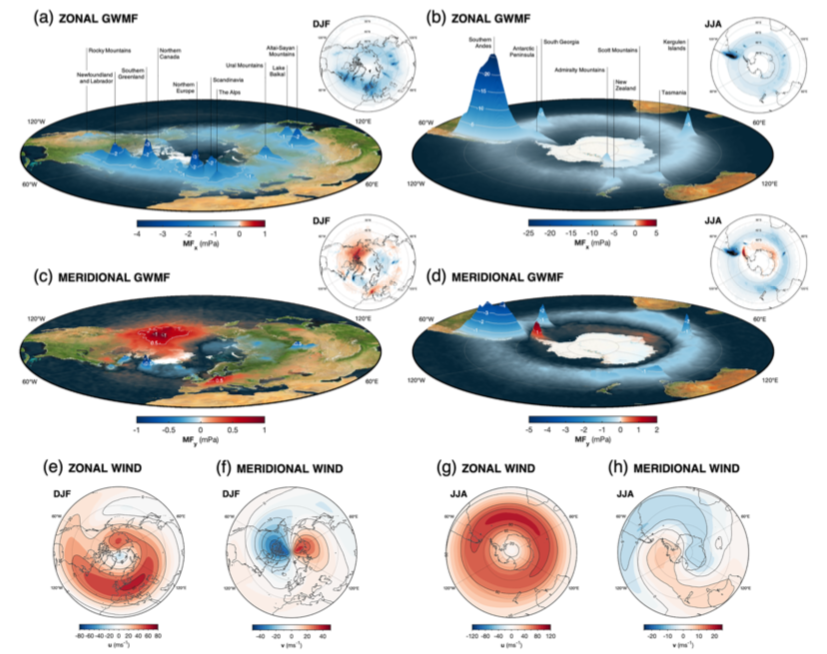
\includegraphics[width=0.99\textwidth]{Figures/hindley_2020_GWMF.png}
    \caption{Stereographic maps of average wintertime zonal (a, b) and meridional (c, d) GWMF near 40 km altitude derived from AIRS/Aqua 3‐D satellite observations for the period 2002–2019. Winter is defined as December–February (June–August) for the Northern (Southern) Hemisphere. GWMF values that are close to zero have been made transparent to reveal the surface features below, and landmarks that lie beneath regions of increased GWMF have been labeled. Inset in the top right of each panel is a stereographic map of the same data but centered on the north and south poles. These inset panels share a color scale with the corresponding 3‐D contours. Panels (e)–(h) show average wintertime zonal and meridional winds at 3 hPa for the period 2002–2019 from ERA5 reanalysis. Taken from \cite{hindley_18year_2020}.}
    \label{fig:hindley_2020_GWMF}
\end{figure*}
%
The increasing number of GW observations from satellites (\cite{hindley_gravity_2019}, \citeyear{hindley_18year_2020}), ground-based lidar systems (\cite{kaifler_lidar_2020} and  \cite{kaifler_compact_2021}), aircraft (\cite{rapp_southtrac-gw_2021} and \cite{fritts_deep_2016}) and  balloons (\cite{plougonven_gravity_2013}) help to constrain GW parameterisations, but also reveal their deficiencies and point out gaps in our current theoretical knowledge on GWs. A phenomenon that was already visible in observations by \textcite{wu_satellite_1996}, but still lacks a conclusive explanation, is a GW belt around 60 \degree S during the austral winter. It is visualized in parts b and d of Fig. \ref{fig:hindley_2020_GWMF} from \textcite{hindley_18year_2020} who provide an extensive overview on seasonally averaged multi-year gravity wave momentum flux (GWMF) derived from satellite observations.


Orography undoubtedly leads to the GW hot spot between $55 \degree$W and $80 \degree$W above the southern Andes and the Antarctic Peninsula,  but it only contributes about $25 \%$ to the total GWMF within the latitude band from $35 \degree$S to $68 \degree$S as stated by \textcite{hindley_18year_2020}. Following \textcite{sato_gravity_2012} and accounting for a far downstream propagation of GWs excited by the Andes, the observable GWMF in the East of the defined longitude region could be allocated to this predominantly local source, too. However, this does not heavily affect the argument of \textcite{hindley_18year_2020} that about $75 \%$ of zonal and meridional GWMF are observed at remaining longitudes over the Southern Ocean mostly peaking around $60 \degree$S (\cite{hindley_18year_2020}).

It has been shown that small, mountainous islands contribute to this oceanic GWMF (\cite{garfinkel_effect_2018}; \cite{mclandress_is_2012}, \cite{alexander_momentum_2009}), but again they only result in local peaks as indicated in Fig. \ref{fig:hindley_2020_GWMF}b. So non-orographic origins of GWs are most likely the reason for the wide-spread, belt-like structure of the GWMF (\cite{hendricks_what_2014}). Jet streams and fronts most likely contribute to the observed momentum flux (\cite{plougonven_internal_2014} and \cite{hendricks_what_2014}) and have also been investigated on the basis of idealized simulations (\cite{osullivan_generation_1995}). \textcite{polichtchouk_sensitivity_2018} analysed the sensitivity of high-resolution atmospheric models to non-orographic GW parameterisations and concluded a significant dependence in the same manner as \textcite{choi_effects_2013} showed that convective gravity wave drag parameterisations (a specific non-orographic source) can have a significant influence on global climate models. In addition, \textcite{jewtoukoff_comparison_2015} were able to assign wave signatures in their balloon observations to non-orographic sources, but so far none of the discussed mechanisms provides a comprehensive explanation of the wide spread observation of GWs over the Southern Ocean in the austral winter and it is still possible that some important mechanisms have not yet been considered.

The gravity wave belt around 60$\degree$S gained crucial relevance since \textcite{mclandress_is_2012} suggested its connection to the longstanding cold pole problem found in nearly all modern GCMs and chemistry climate models (CCMs). During the southern hemisphere winter months a polar vortex or polar night jet (PNJ) develops around 60$\degree$S high up in the stratosphere characterized by strong zonal westerly winds. GCMs and CCMs overestimate this PNJ, which also entails lower stratospheric temperatures over the pole compared to observations (\cite{butchart_multimodel_2011}, \cite{geller_comparison_2013} and \cite{eyring_sparc_2010}). As a result, the polar vortex breaks down too late in the spring with significant consequences on, for example, the simulated ozone trends in the Antarctic middle stratosphere (\cite{stolarski_ozone_2006}). The Antarctic ozone hole persists too long into the late spring and since Antarctic ozone depletion is the primary driver of recent southern hemisphere summertime climate change (e.g. \cite{arblaster_contributions_2006}), a delay in the vortex breakdown impacts the timing of the simulated tropospheric response.

\textcite{mclandress_is_2012} showed through their simulations that missing gravity wave drag from parameterisations can explain this substantial zonal wind bias around 60°S and the directly related "cold pole". A deeper understanding of the key processes that lead to the observed gravity wave belt during the austral winter could significantly improve GW parameterisations and ultimately improve long-term climate predictions through more realistic and robust GCMs. 

% include polar vortex image to show zonal wind distribution.

% or if it ultimately is a superposition of all known sources.

% temperature measurements of satellite
% in the vicinity of the 60°S belt

%%%
% excitation, propagation and dissipation
% \textcite{}
% \citeyear{}
%%%

\subsection{The excitation of GWs above tropopause depressions}
\label{sec:excitation}

As outlined in the previous section, non-orographic GW sources have already been investigated from various perspectives, but are not yet able to fully explain the consistent, wide-spread appearance of GWs around 60$\degree$S. Based on observations and the analysis of high-resolution ERA5 data, \textcite{dornbrack_stratospheric_2021} are currently proposing a new mechanism that has the potential to fill this gap. They suggest the excitation of GWs above tropopause depressions (TDs) in the stratosphere just like they would appear above surface obstacles in the troposphere. 

Though various definitions of the tropopause exist, all rely on abrupt changes in physical or chemical properties when transitioning from a weakly stratified troposphere ($N^2 \approx$ 1$\cdot 10^{-4}$\SI{}{s^{-2}}) to a comparatively strongly stratified stratosphere ($N^2 \approx$ 4$\cdot 10^{-4}$\SI{}{s^{-2}}; \cite{birner_fine-scale_2006}). Common definitions are based on the thermal stratification (negative temperature lapse rate in the troposphere, positive  lapse rate in the stratosphere; \cite{wmo_meteorology_1957}), refer to the dynamical tropopause using Ertel's potential vorticity (\cite{wmo_atmospheric_1986}) or rely on chemical tracers like ozone. Despite fundamental differences in those approaches, each supports the simplification of treating the tropopause as an impermeable boundary, which is definitely not true, but a good approximation for idealized investigations. 

In the vicinity of jet streams or upper level frontal zones and associated with baroclinic processes the extratropical tropopause now  experiences deflections or even undergoes a folding process as visualized in Fig. \ref{fig:skerlakFold}. Dry stratospheric air penetrates down into the troposphere and folds underneath the warm air towards the equator (here northward for southern hemisphere) for deep depressions. % Potentially warmer stratospheric air
%
\begin{figure*}[h]
    \centering
    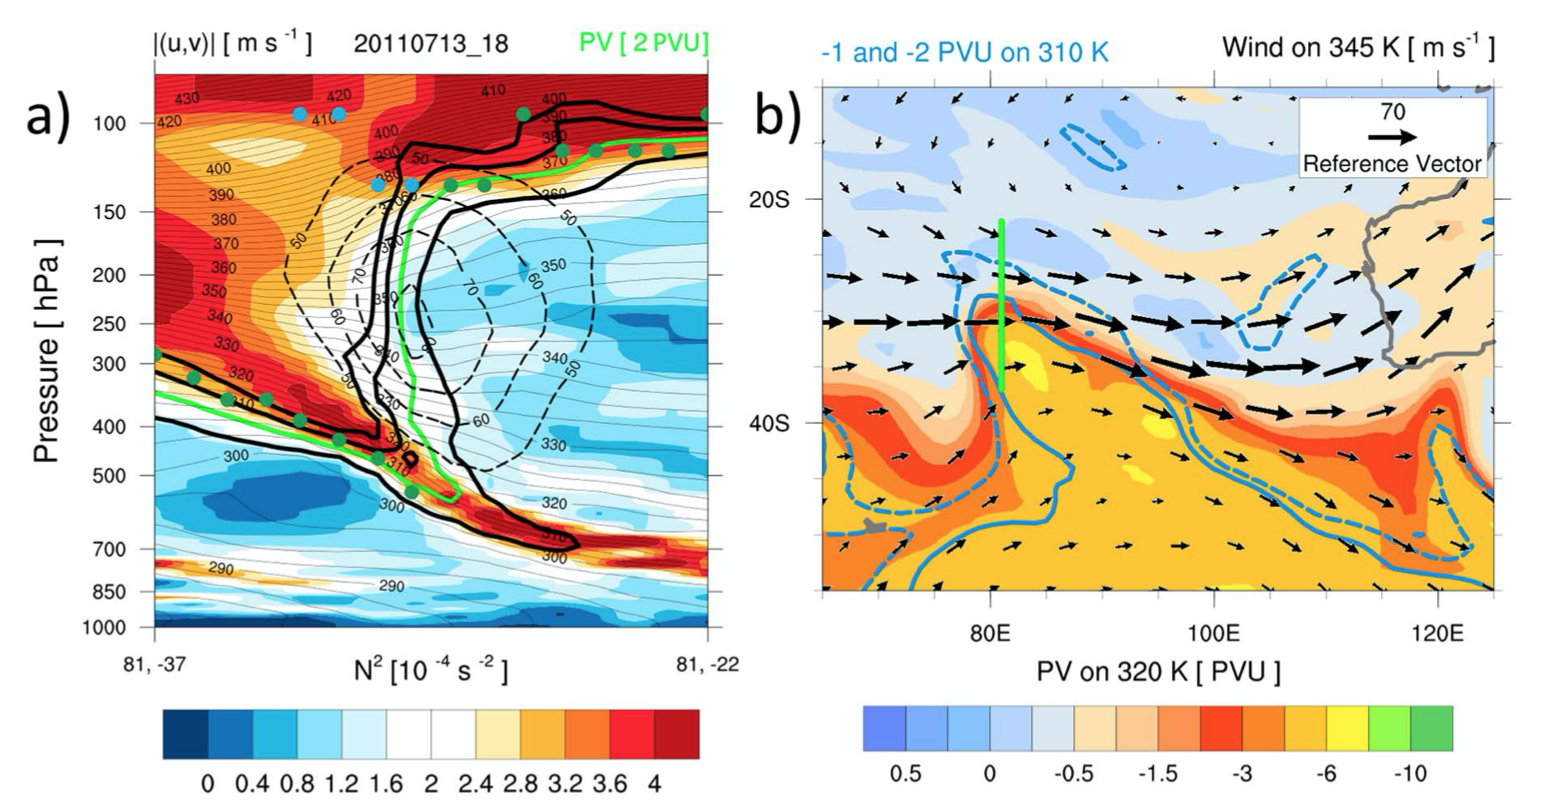
\includegraphics[width=0.99\textwidth]{Figures/Skerlak_Fold.png}
    \caption{Example of a deep tropopause fold near the subtropical jet west of Australia at 18 UTC on 13 July 2011. The vertical cross section shown in Figure 2a is aligned along 81$\degree$E from 37S$\degree$ to 22$\degree$S (green line segment in Figure 2b). Displayed are (a) the squared Brunt-Vaisala frequency ($N^2$, colored), potential vorticity (-1 to -4 PVU, thick solid lines, -2 PVU in green, rest in black), the WMO first and second tropopauses (green and blue solid circles, respectively), horizontal wind speed (in \SI{1}{\meter\second^{-1}}, dashed contours), and isentropes (in K, thin contours) and (b) PV on 320 K (colored, in PVU), contours of PV on 310 K at -1 PVU and -2 PVU (dashed and solid blue, respectively), and horizontal wind speed on 345K (reference vector in the top right, in \SI{1}{\meter\second^{-1}}). The West Coast of Australia is visible as grey contour. Taken from \cite{skerlak_tropopause_2015}.}
    \label{fig:skerlakFold}
\end{figure*}
%
The shape of the TD and especially the vertical extend of the prominent tongue of stratospheric air can vary significantly depending on the large scale flow conditions and strength of the upper level frontal system. This has already been discussed extensively from an observational (e.g. \cite{shapiro_further_1978} and \cite{keyser_review_1986}) and model (\cite{skerlak_tropopause_2015}) perspective. Fortunately, the excitation of GWs above such a depression might not be very sensitive to the fold's shape far below the tropopause. Isentropes, that are deflected downwards, but rise again on the other side of the depression (e.g. 360-\SI{390}{\kelvin} in Fig. \ref{fig:skerlakFold}a) are much more interesting for the proposed mechanism considering its similarity to flow over orography. Additionally, the zonal shape of the depression is more relevant for the GW forcing. This along-stream cross section (orthogonal on \ref{fig:skerlakFold}a) was rarely discussed in relevant publications, since the main folding process happens in the cross-stream direction. Based on the ERA5 case study conducted by \textcite{dornbrack_stratospheric_2021} (Fig. \ref{fig:RF25_waves}), the zonal width at half maximum of the propagating TD can be estimated between $4 \degree$ and $8 \degree$ in zonal direction, which transfers to $a=240-$\SI{480}{\kilo\meter}
($1\degree \approx$ \SI{63}{\kilo\meter} at $55 \degree$S). 

Following estimates based on idealized scenarios (constant background wind $U$ and Brunt–Väisälä frequency $N$) such 'mountain widths' are expected to excite waves within the hydrostatic regime. Towards the wider end of $a$ the advection time for an air parcel to pass over the mountain $\tau_a = \frac{a}{U}$ is even comparable in magnitude to the period of inertial oscillation due to Earth’s rotation ($\tau_f = \frac{2 \pi}{f}$) with the Coriolis parameter $f \approx 10^{-4}$\SI{}{\second^{-1}} for mid-latitudes. So the Rossby number
% Thus, the time it takes for a fluid particle to cross the ridge is much larger than the period of a buoyancy oscillation
% We notice that τf /τa = 2πU/(fa) ≈ Ro
\begin{equation}
    Ro = \frac{U}{f a} \approx \frac{\tau_f}{\tau_a} \approx 2 \pi
\end{equation}
%
is close to $O(1)$ and Coriolis forces can no longer be neglected. Together with the buoyancy forces they act together as restoring forces resulting in both horizontal and vertical oscillations, which are called hydrostatic inertia-gravity waves (e.g. \cite{gill_atmosphere-ocean_1982} and \cite{lin_mesoscale_2007}).
% Froude number for linear non-linearity with height!!
% $L N U^{-1}$
% should be 60 m/s wind or 100km wide depression for hydrostatic scenario

A major difference of potential GWs above TDs to classic mountain waves is the transient nature of their source. \textcite{pfister_gravity_1993} already investigated the propagation of waves in the stratosphere due to a transient forcing by exposing the background flow to a time-varying obstacle, but only lifted and receded the bottom of the stratosphere. A tropopause fold travels eastward with the phase speed of the Rossby wave, so the relative motion of the stratospheric air aloft with respect to the propagation of the fold is responsible for the excitation of the GWs. The increasing wind speed with height due to the PNJ, which is already important for the propagation of the waves, is, therefore, important for their excitation, too.

\subsection{The propagation of GWs above tropopause depressions}
\label{sec:propagation}

Considering the hydrostatic nature of GWs excited by TDs, the strongest wave signal should more or less appear directly above a propagating depression. In fact, \textcite{dornbrack_stratospheric_2021} observed exactly this feature in ERA5 data (Fig. \ref{fig:RF25_waves}), when analysing lidar measurements from DEEPWAVE research flight 25. Clear wave signals are observed directly above the tropopause fold for multiple points in time. This inspires confidence in the proposed mechanism and suggests that GWs can be observed along the whole path of the baroclinic system responsible for the depression.
%
\begin{figure*}[h]
    \centering
    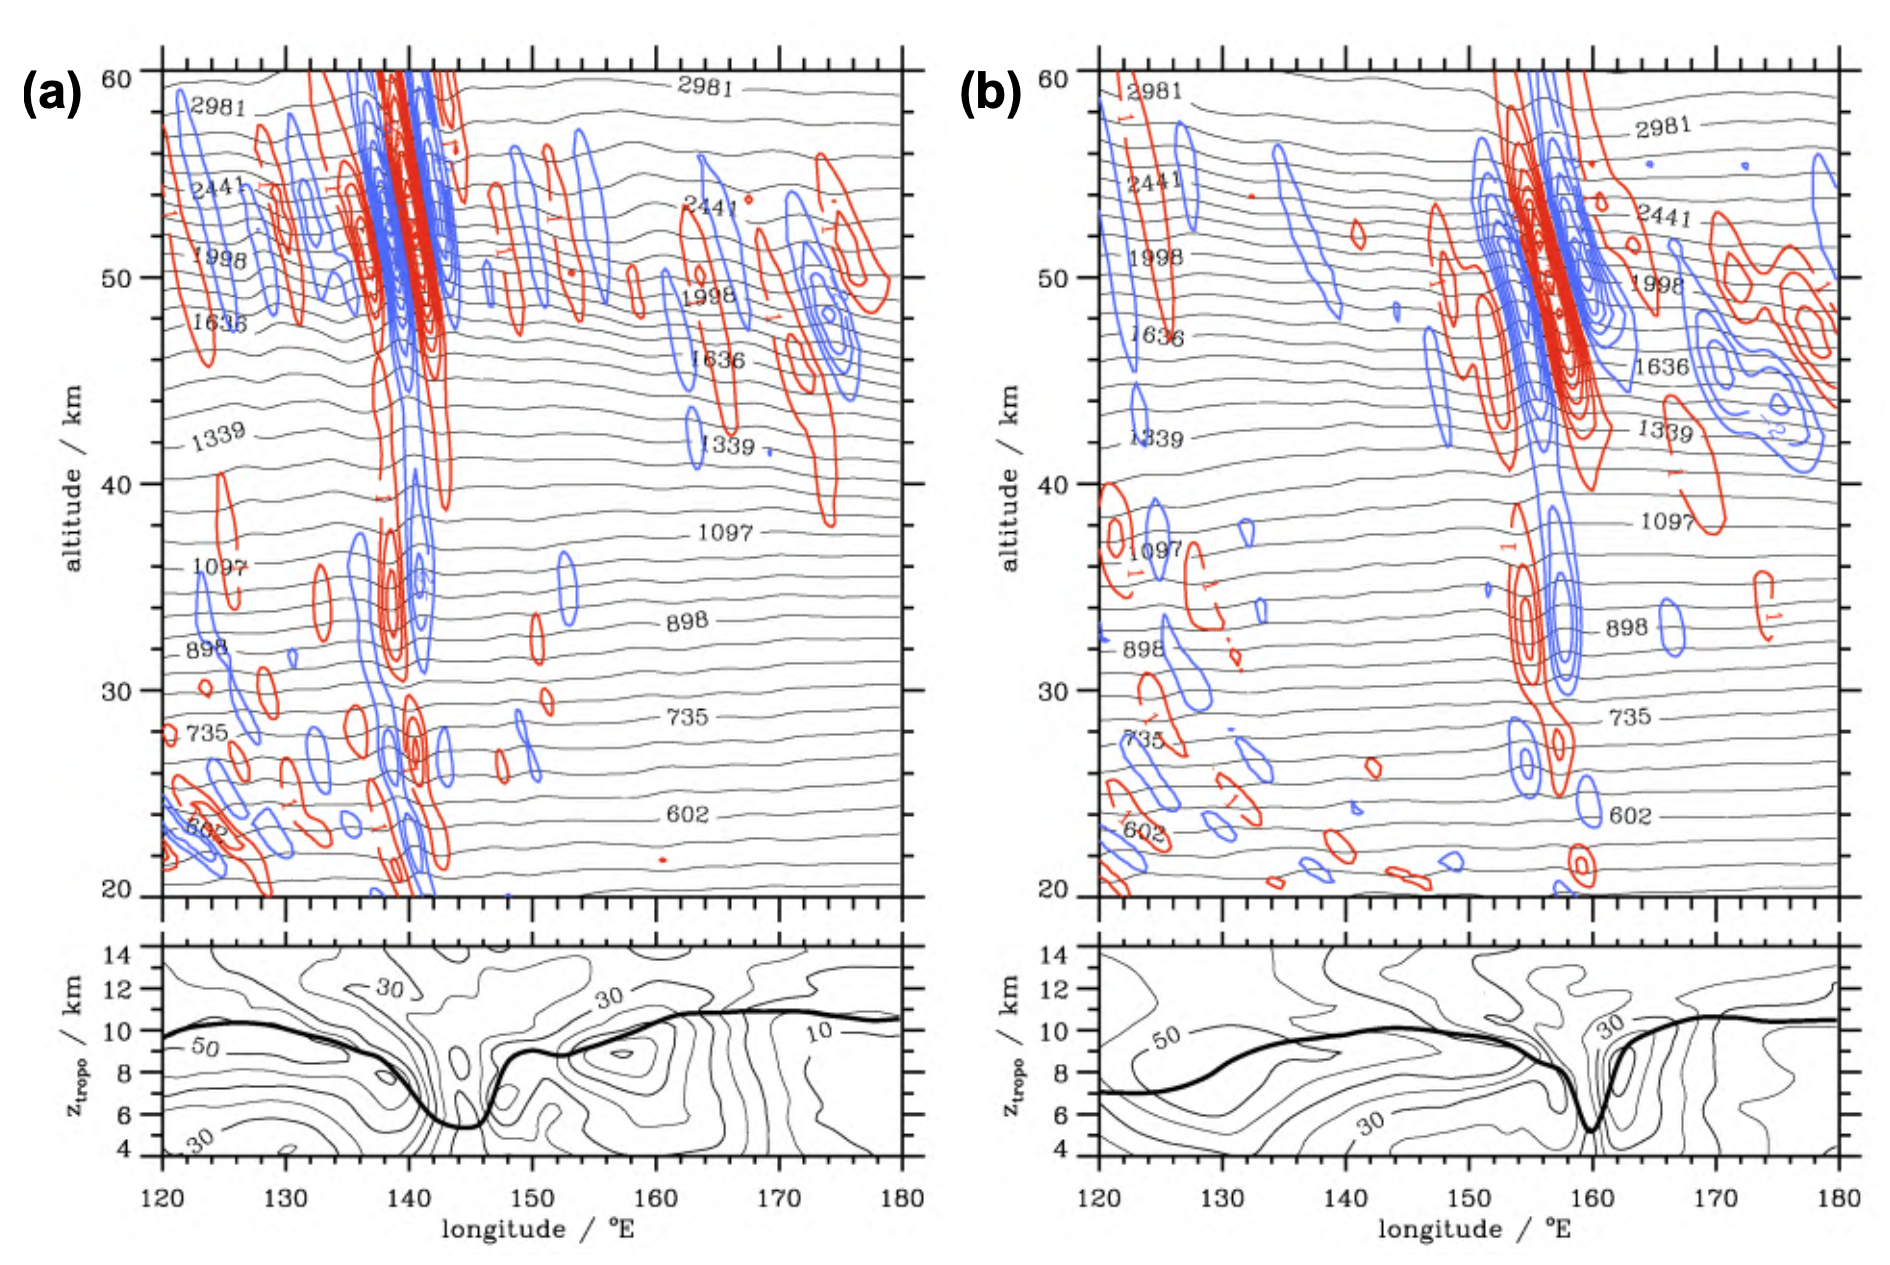
\includegraphics[width=0.99\textwidth]{Figures/RF25_waves.png}
    \caption{Temperature perturbations (K, red and blue contour lines) and potential temperature (K, black lines in logarithmic scaling) along 55$\degree$S on 17 July 2014 15 UTC (a) and 18 July 2014 09 UTC (b). The bottom panels depict the height of the dynamical tropopause (thick black lines, meridional average from 52.5$\degree$S to 57.5$\degree$S) and the horizontal wind (\SI{}{\meter\second^{-1}}, thin black lines) at the same instances. Data: One hourly ERA5 data. Taken from Dörnbrack et al. (2021).}
    \label{fig:RF25_waves}
\end{figure*}
%
Now, the last piece to the puzzle for explaining the wave belt above the Southern Ocean during the austral winter in Fig. \ref{fig:hindley_2020_GWMF}b and \ref{fig:hindley_2020_GWMF}d is the meridional propagation of GWs in the stratosphere. This is important, because especially in the southern hemisphere pronounced frontal systems are not deviating significantly from a latitude band around 50$\degree$S (\cite{skerlak_tropopause_2015}) though GWs are observed frequently further south.

Two mechanisms are at hand concerning this meridional propagation. At first, the orientation of the TDs is rarely exactly North-South resulting in an inclined wave vector with respect to the predominantly westerly flow in the upper stratosphere. The wave vector defines the propagation direction, so this mechanism is always present and relevant as soon as tilted obstacles are in place as discussed by \textcite{preusse_space-based_2002} for GWs excited by the Andes at similar latitudes. The second process is based on ray-tracing theory and was first discussed and applied by \textcite{dunkerton_dunkerton_inertiagravity_1984}. It describes the modification of the meridional (horizontal) wavenumber by the background wind field with
%
\begin{equation}
    \frac{dl}{dt} = -(k \frac{\partial U}{\partial y} + l \frac{\partial V}{\partial y} + \frac{\beta f}{\hat{\omega}})
    \approx -k \frac{\partial U}{\partial y}.
    \label{equ:meridionalRefraction}
\end{equation}
%
In a simplified scenario the time rate of change of the meridional wavenumber $l$ along the ray is proportional to the meridional gradient of the background wind $U$ and the zonal wavenumber $k$. In other words, horizontal wind shear develops a meridional component of the wave vector even in the case of a purely zonal initial propagation. In general, this phenomenon leads to a refraction of internal GWs into the southern hemispheric PNJ at 60$\degree$S, which has already been described by a number of publications (e.g. \cite{dunkerton_dunkerton_inertiagravity_1984}, \cite{preusse_space-based_2002}, \cite{sato_origins_2009}, \cite{sato_gravity_2012}, \cite{ehard_horizontal_2017} and \cite{jiang_stratospheric_2019}). \textcite{jiang_stratospheric_2019} further add, that waves are elongated towards the stronger background wind (towards the center of the PNJ) and shortened on the opposite side with weaker winds.

\subsection{Research goals and outline}
\label{sec:goals}
%
In the end, both described mechanisms play an important role for the meridional propagation of GWs. Together with the regular appearance of Rossby wave trains (baroclinic systems involving TDs) at middle latitudes in the southern hemisphere, these processes could provide a conclusive explanation for the widespread and patchy stratospheric GW activity all the way around the Southern Ocean shown in Fig. \ref{fig:hindley_2020_GWMF}b and \ref{fig:hindley_2020_GWMF}d. It is the goal of the proposed thesis to further investigate the relevant processes related to GWs above tropopause depressions through idealized simulations and eventually provide first answers on its relevance for explaining the discussed GW belt above the Southern Ocean. More specifically, the Master's thesis shall answer the following research questions:
%
\begin{enumerate}
    \item How sensitive is the excitation and propagation of GWs above TDs to the shape of the depression (depth, width, asymmetry)?
    \item Which wave regimes are present above propagating TDs and what wavelengths and amplitudes do we expect?
    \item What is the contribution of a tilted TD (leading to an inclined wave vector) to a meridional propagation of GWs?
    \item What is the contribution of horizontal wind shear in the stratosphere to a meridional propagation of GWs?
    % \item How significant is the effect of the Coriolis force in 2D and 3D simulations?
\end{enumerate}

%% In baroclinic simulation advection of waves meridionally possible!!!

% Stationary synoptic patterns like blocks are rare in the southern hemisphere, because of 

%% NOTES %%
% include figure and description
% hydrostatic waves (include figure from RF25 of waves above depression)

% It is clear that the flow regime above a TD is much more complicated than a zonal overflow of an elongated mountain ridge, which produces the expected hydrostatic waves aloft. Three dimensional Furthermore, the fold itself travels eastward with the phase speed of the Rossby

% impermeable boundary
% shear wind rotation with height to strong zonal wind 

% The World Meteorological Organization defines the tropopause as the lowest level where the abso- lute value of the temperature lapse rate decreases to 2K/km. or less, with the average lapse rate between this level and all higher levels within 1.2 mi. (2 km.) not exceeding 2K/km. The dynamical tropopause is defined in terms of sharp changes in the potential vor- ticity (much higher in the stratosphere), which mea- sures stratification and rotation of the air masses. An abrupt increase (decrease) with height of the ozone (water vapor) mixing ratio indicates the presence of the chemical tropopause.

% thermal definition
% dynamic definition potential temperature and pressure on the dynamic tropopause (defined here as the 1.5 × 10−6 m2 K kg−1 s−1, hereafter 1.5 PVU, Ertel PV surface)
% chemical definition

% thermal fields and wind fields

% bush vertical / horizontal aspect ratio of 0.06 penetrates the troposphere

% \cite{clark_convectively_1986} above inversion layer?? 